\documentclass[12pt, a4paper]{article}

% ─── 编码与字体 ───────────────────────────────────────────────────────────────
\usepackage[UTF8]{ctex}
\usepackage[T1]{fontenc}
\usepackage{lmodern}

% ─── 页面与版式 ───────────────────────────────────────────────────────────────
\usepackage[margin=2.5cm]{geometry}
\usepackage{microtype}
\usepackage{parskip}
\setlength{\parindent}{0pt}

% ─── 数学 ─────────────────────────────────────────────────────────────────────
\usepackage{amsmath, amssymb, amsthm}
\usepackage{mathtools}
\usepackage{bm}

% ─── 表格与图形 ───────────────────────────────────────────────────────────────
\usepackage{booktabs}
\usepackage{array}
\usepackage{graphicx}
\usepackage{float}
\usepackage{tikz}
\usetikzlibrary{arrows.meta, positioning, shapes.geometric}

% ─── 代码高亮 ─────────────────────────────────────────────────────────────────
\usepackage{listings}
\usepackage{xcolor}

\definecolor{leanblue}{RGB}{0, 80, 160}
\definecolor{leangreen}{RGB}{0, 120, 60}
\definecolor{leangray}{RGB}{110, 110, 110}
\definecolor{leanpurple}{RGB}{120, 40, 140}
\definecolor{leanred}{RGB}{180, 40, 40}
\definecolor{codebg}{RGB}{248, 248, 252}

\lstdefinelanguage{Lean4}{
  keywords={theorem, lemma, def, noncomputable, structure, where, by, have, set, haveI,
            exact, apply, intro, induction, simp, rw, ring, linarith, nlinarith,
            field_simp, gcongr, calc, fun, let, match, variable, import, open,
            namespace, end, section, universe, forall, exists, if, then, else,
            return, do, mut, instance, class, extends, with, in, at, from,
            rfl, congr, positivity, norm_num, push_neg, contrapose, constructor},
  keywordstyle=\color{leanblue}\bfseries,
  morekeywords={[2]{Measurable, Integrable, IsProbabilityMeasure, IndepFun, iIndepFun,
                    MeasureTheory, ProbabilityTheory, ConvexOn, StrongConvexOn,
                    HasGradientAt, LipschitzWith, Filtration, Adapted,
                    integral, iSup, Finset, Set, Measure, BorelSpace}},
  keywordstyle={[2]\color{leanpurple}},
  comment=[l]{--},
  morecomment=[s]{/-}{-/},
  commentstyle=\color{leangray}\itshape,
  stringstyle=\color{leanred},
  literate=
    {→}{{$\to$}}1
    {←}{{$\leftarrow$}}1
    {⟹}{{$\Rightarrow$}}1
    {∀}{{$\forall$}}1
    {∃}{{$\exists$}}1
    {⟪}{{$\langle$}}1
    {⟫}{{$\rangle$}}1
    {∈}{{$\in$}}1
    {∉}{{$\notin$}}1
    {⊆}{{$\subseteq$}}1
    {≤}{{$\le$}}1
    {≥}{{$\ge$}}1
    {≠}{{$\ne$}}1
    {‖}{{$\|$}}1
    {‹}{{$\langle$}}1
    {›}{{$\rangle$}}1
    {⨆}{{$\bigsqcup$}}1
    {ℕ}{{$\mathbb{N}$}}1
    {ℝ}{{$\mathbb{R}$}}1
    {Ω}{{$\Omega$}}1
    {σ}{{$\sigma$}}1
    {η}{{$\eta$}}1
    {μ}{{$\mu$}}1
    {ξ}{{$\xi$}}1
    {•}{{$\cdot$}}1,
  backgroundcolor=\color{codebg},
  basicstyle=\ttfamily\small,
  breaklines=true,
  frame=single,
  framesep=4pt,
  rulecolor=\color{gray!40},
  tabsize=2,
  showstringspaces=false,
}
\lstset{language=Lean4}

% ─── 超链接 ───────────────────────────────────────────────────────────────────
\usepackage{hyperref}
\hypersetup{
  colorlinks=true,
  linkcolor=leanblue,
  citecolor=leangreen,
  urlcolor=leanblue,
}

% ─── 定理环境 ─────────────────────────────────────────────────────────────────
\newtheorem{theorem}{定理}[section]
\newtheorem{lemma}[theorem]{引理}
\newtheorem{corollary}[theorem]{推论}
\newtheorem{definition}[theorem]{定义}
\newtheorem{remark}[theorem]{注记}
\newtheorem{observation}[theorem]{观察}

% ─── 自定义命令 ───────────────────────────────────────────────────────────────
\newcommand{\E}{\mathbb{E}}
\newcommand{\R}{\mathbb{R}}
\newcommand{\N}{\mathbb{N}}
\newcommand{\gradF}{\nabla f}
\newcommand{\gradL}{\nabla L}
\newcommand{\ip}[2]{\langle #1,\, #2 \rangle}
\newcommand{\norm}[1]{\left\| #1 \right\|}
\newcommand{\wstar}{w^*}
\newcommand{\lean}[1]{\texttt{#1}}
\newcommand{\file}[1]{\textbf{\texttt{#1}}}

% ─── 标题 ─────────────────────────────────────────────────────────────────────
\title{%
  \textbf{SGD 收敛性的 Lean 4 形式化分析}\\[0.5em]
  \large 证明架构、基础设施设计与 Mathlib 边界研究
}
\author{基于 \texttt{/SGD} 代码库的深度分析}
\date{\today}

% ═════════════════════════════════════════════════════════════════════════════
\begin{document}
% ═════════════════════════════════════════════════════════════════════════════

\maketitle
\tableofcontents
\newpage

% ─────────────────────────────────────────────────────────────────────────────
\section{引言}
% ─────────────────────────────────────────────────────────────────────────────

\subsection{项目背景}

随机梯度下降（Stochastic Gradient Descent，SGD）是现代机器学习的核心算法之一。
其收敛性分析已在数学文献中被充分研究，但将这些分析\emph{机器验证}——即在交互式证明助手中
给出完整的形式化证明——仍是数学形式化领域的前沿挑战。

本代码库（\texttt{/SGD}）在 Lean 4 + Mathlib 框架下，对实 Hilbert 空间 $E$ 上的 SGD 算法
给出了三种经典收敛定理的完整形式化证明，覆盖了从非凸到强凸的完整难度谱系。

\subsection{主要结果概览}

\begin{table}[H]
\centering
\caption{三种 SGD 收敛定理}
\begin{tabular}{lccc}
\toprule
\textbf{定理} & \textbf{条件} & \textbf{收敛率} & \textbf{文件位置} \\
\midrule
\lean{sgd\_convergence\_nonconvex} & $L$-光滑 & $O(1/\sqrt{T})$，$\E\norm{\gradF(w_t)}^2$ & Main.lean §8 \\
\lean{sgd\_convergence\_convex}    & $L$-光滑 + 凸 & $O(1/\sqrt{T})$，$\E[f(w_t)-f^*]$ & Main.lean §9 \\
\lean{sgd\_convergence\_strongly\_convex} & $L$-光滑 + $\mu$-强凸 & 线性收敛 & Main.lean §10 \\
\bottomrule
\end{tabular}
\end{table}

每个收敛定理均采用\textbf{两层结构}：
\begin{enumerate}
  \item \textbf{一步引理}：对每次迭代建立期望进展的精确上界。
  \item \textbf{收敛定理}：对一步引理求和/递推，通过望远镜求和或归纳得到最终界。
\end{enumerate}

\subsection{文件架构}

整个代码库由四个 Lean 文件组成，其依赖关系如下：

\begin{center}
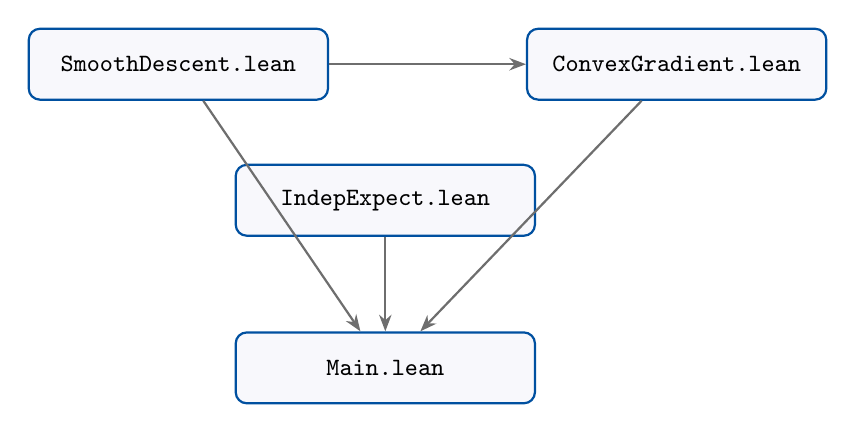
\begin{tikzpicture}[
  node distance=1.5cm and 2.5cm,
  box/.style={rectangle, draw=leanblue, thick, rounded corners=4pt,
              minimum width=3.8cm, minimum height=0.9cm,
              font=\small\ttfamily, fill=codebg},
  arrow/.style={-{Stealth[length=6pt]}, thick, color=leangray}
]
  \node[box] (smooth) {SmoothDescent.lean};
  \node[box, right=of smooth] (convex) {ConvexGradient.lean};
  \node[box, below right=0.8cm and -1.2cm of smooth] (indep) {IndepExpect.lean};
  \node[box, below=1.2cm of indep] (main) {Main.lean};

  \draw[arrow] (smooth) -- (main);
  \draw[arrow] (smooth) -- (convex);
  \draw[arrow] (convex) -- (main);
  \draw[arrow] (indep) -- (main);
\end{tikzpicture}
\end{center}

\begin{itemize}
  \item \file{SmoothDescent.lean}：$L$-光滑函数的解析工具（FTC + 二次上界）
  \item \file{ConvexGradient.lean}：凸/强凸函数的一阶条件（依赖 SmoothDescent）
  \item \file{IndepExpect.lean}：独立性与期望分解的测度论工具
  \item \file{Main.lean}：SGD 定义、自然滤子、独立性引理、三个收敛定理
\end{itemize}

% ─────────────────────────────────────────────────────────────────────────────
\section{证明的核心难点与瓶颈}
% ─────────────────────────────────────────────────────────────────────────────

\subsection{非正式证明与形式化之间的鸿沟}

教材中 SGD 收敛分析的核心步骤通常写作：

\begin{quote}
``对 $\xi_t$ 取条件期望，利用 $w_t$ 与 $\xi_t$ 的独立性和梯度的无偏性，得到
$\E[\ip{\nabla f(w_t)}{g_t}] = \E[\norm{\nabla f(w_t)}^2]$。''
\end{quote}

这句话在非正式叙述中是完全平凡的。然而，要在 Lean 4 中形式化这一步，需要将其分解为
\textbf{至少五个独立的形式化步骤}：

\begin{enumerate}
  \item \textbf{证明 $w_t \perp \xi_t$}：$w_t$ 只依赖 $\xi_0,\ldots,\xi_{t-1}$，必须通过
        自然滤子 $\mathcal{F}_t = \sigma(\xi_0,\ldots,\xi_{t-1})$ 和 \lean{iIndepFun} 的
        $\sigma$-代数格推理正式建立（见 \lean{sgdProcess\_indepFun\_xi}，Main.lean 第 171--209 行）。

  \item \textbf{将联合分布分解为乘积测度}：利用 Mathlib 的等价刻画
        \lean{indepFun\_iff\_map\_prod\_eq\_prod\_map\_map}，将
        \[
          P \circ (w_t, \xi_t)^{-1} = (P \circ w_t^{-1}) \otimes \nu
        \]
        作为显式命题证明（IndepExpect.lean 第 61--62 行）。

  \item \textbf{应用 Bochner-Fubini 定理}：通过 \lean{integral\_prod} 将乘积测度上的积分
        分解为迭代积分，需要显式验证可积性条件。

  \item \textbf{应用无偏性假设}：在 Fubini 之后的内层积分中，调用
        $\int_S \nabla L(w, s)\, d\nu(s) = \nabla f(w)$，通过 \lean{integral\_inner} 将
        $h(w)$ 拉出内积后应用。

  \item \textbf{将结果推回原测度}：通过 \lean{integral\_map} 将
        $P \circ w_t^{-1}$ 上的积分还原到 $P$ 上的积分。
\end{enumerate}

这五步的总实现体现在 IndepExpect.lean 的两个核心定理中，构成了整个证明库的测度论核心。

\subsection{$\sigma$-代数格推理的形式化负担}

以 \lean{sgdProcess\_indepFun\_xi} 为例，其证明展示了$\sigma$-代数格推理的繁琐性：

\begin{lstlisting}
lemma sgdProcess_indepFun_xi ... (t : N) :
    IndepFun (sgdProcess ... t) (x t) P := by
  -- 自然滤子 F_t = sup_{j < t} sigma(x_j)
  set F := sgdFiltration x hx_meas
  -- process t 关于 F t 可测
  have h_adapted : Measurable[F t] (sgdProcess ... t) := ...
  -- comap(process t) <= F t
  have h_comap_le : comap(process t) <= F t := ...
  -- F t 与 comap(x t) 独立（关键步骤）
  have h_filt_indep : Indep (F t) (comap (x t)) P := by
    -- 利用指标集不相交：{j | j < t} 与 {t} 不相交
    have h_disj : Disjoint {j | j < t} {t} := ...
    exact indep_iSup_of_disjoint h_le h_iIndep h_disj
  -- 单调性：comap(process t) <= F t => 继承独立性
  exact indep_of_indep_of_le_left h_filt_indep h_comap_le
\end{lstlisting}

注意这段代码的数学内容（``wt 只依赖过去的样本''）是完全平凡的，
但其形式化需要在 \lean{MeasurableSpace} 的上确界格（\lean{iSup}）上做精确的格运算，
并显式处理 \lean{comap}、\lean{Indep}、\lean{iIndep} 三个不同层次的独立性概念之间的关系。

\subsection{可积性的全量追踪}

Lean 中每次使用积分线性性（$\int(f+g) = \int f + \int g$）都需要提供 $f$ 和 $g$ 的
可积性证明。这导致每个一步引理的函数签名携带大量 \lean{Integrable} 假设。
以 \lean{stochastic\_descent\_nonconvex} 为例，其签名需要：

\begin{lstlisting}
(h_int_ft  : Integrable (fun o => f (process t o)) P)
(h_int_ft1 : Integrable (fun o => f (process (t+1) o)) P)
(h_int_inner : Integrable (fun o =>
    <gradF (process t o), gradL (process t o) (x t o)>_R) P)
(h_int_sq   : Integrable (fun o =>
    ||gradL (process t o) (x t o)||^2) P)
(h_int_gF_sq : Integrable (fun o =>
    ||gradF (process t o)||^2) P)
\end{lstlisting}

这七个可积性假设在教材中被隐式假定，而在 Lean 中必须由调用方逐一提供。
更根本的问题是，Mathlib 目前缺乏针对 SGD 迭代结构的\textbf{自动可积性传播}工具。

\subsection{期望层面的不等式推理}

形式化证明中大量出现对积分的估计，例如：
\[
  \int \ip{\nabla f(w_t)}{\nabla f(w_t)}\, dP \leq \int \sigma^2\, dP
\]
这类不等式不能直接被 \lean{linarith} 处理，需要手动调用 \lean{integral\_mono}，
并为每次调用提供被积函数的可测性和被积函数的逐点不等式。
在随机优化中，这类期望不等式链远多于普通标量不等式链，显著增加了证明的技术负担。

% ─────────────────────────────────────────────────────────────────────────────
\section{新建基础设施的作用与设计}
% ─────────────────────────────────────────────────────────────────────────────

三个辅助文件共同构成了一个\textbf{随机优化分析的小型基础库}。
这个库在 Mathlib 主库中是缺失的，是本代码库得以完成完整形式化证明的关键。

\subsection{\file{SmoothDescent.lean}：L-光滑的解析基础设施}

\subsubsection{背景：Mathlib 的现有工具与缺口}

Mathlib 提供了 \lean{HasGradientAt}（函数在一点处有梯度）和 \lean{LipschitzWith}（Lipschitz
连续性），但没有将二者连接起来的关键结果：$L$-光滑函数的二次上界。

\subsubsection{定理 1：沿线段的微积分基本定理}

\begin{definition}
设 $f : E \to \R$ 在每点 $w$ 处有梯度 $\nabla f(w)$，$\nabla f$ 连续。则对任意 $x, d \in E$：
\[
  f(x + d) - f(x) = \int_0^1 \ip{\nabla f(x + t \cdot d)}{d}\, dt
\]
\end{definition}

该结果（\lean{integral\_inner\_gradient\_segment}）在 Mathlib 中完全缺失。证明分两步：
\begin{enumerate}
  \item 证明 $\varphi(t) = f(x + t \cdot d)$ 在每个 $t$ 处有导数
        $\ip{\nabla f(x + t\cdot d)}{d}$（通过 \lean{hasDerivAt\_comp\_lineSegment}，
        利用 $f$ 的 Fréchet 导数与线段参数化的链式法则，再经 \lean{toDual\_apply\_apply} 转换）。
  \item 将标量版本的微积分基本定理 \lean{intervalIntegral.integral\_eq\_sub\_of\_hasDerivAt}
        应用于 $\varphi$。
\end{enumerate}

\subsubsection{定理 2：L-光滑二次上界}

\begin{theorem}[\lean{lipschitz\_gradient\_quadratic\_bound}]
若 $\nabla f$ 是 $L$-Lipschitz 的，则对任意 $x, d \in E$：
\[
  f(x + d) \leq f(x) + \ip{\nabla f(x)}{d} + \frac{L}{2} \norm{d}^2
\]
\end{theorem}

\begin{proof}[证明思路]
将线段 FTC 的被积函数拆分：
\[
  \ip{\nabla f(x + t\cdot d)}{d} = \ip{\nabla f(x)}{d} + \underbrace{\ip{\nabla f(x+t\cdot d) - \nabla f(x)}{d}}_{\text{余项}}
\]
对余项应用 Cauchy-Schwarz + Lipschitz 条件：
\[
  \ip{\nabla f(x+t\cdot d) - \nabla f(x)}{d} \leq \norm{\nabla f(x+t\cdot d) - \nabla f(x)} \cdot \norm{d}
  \leq L \cdot t \cdot \norm{d}^2
\]
对 $t \in [0,1]$ 积分，得余项贡献 $\leq \int_0^1 L \cdot t \cdot \norm{d}^2\, dt = \frac{L}{2}\norm{d}^2$。\qed
\end{proof}

该定理是非凸收敛定理中 \lean{descent\_lemma} 的直接来源。

\subsection{\file{ConvexGradient.lean}：凸函数的几何基础设施}

\subsubsection{背景：多维凸一阶条件的缺失}

Mathlib 有 \lean{ConvexOn}（凸函数）和 \lean{StrongConvexOn}（强凸函数）的完整定义，
以及一维情形的切线不等式。但\textbf{多维（Hilbert 空间）版本的一阶最优性条件}缺失：
\[
  f \text{ 凸} + \text{可微} \implies f(y) \geq f(x) + \ip{\nabla f(x)}{y - x}
\]

\subsubsection{定理 3：凸函数的一阶条件}

\begin{theorem}[\lean{convex\_first\_order\_condition}]
设 $f : E \to \R$ 在 $\text{univ}$ 上凸，且 $\nabla f$ 处处存在，则对任意 $x, y \in E$：
\[
  f(y) \geq f(x) + \ip{\nabla f(x)}{y - x}
\]
\end{theorem}

\begin{proof}[证明思路]
构造 $g(t) = f(x + t \cdot (y-x))$。通过 \lean{ConvexOn.comp\_affineMap} 证明 $g$
在 $\R$ 上凸（归约到标量情形）。对 $g$ 应用 Mathlib 的标量版本切线不等式
\lean{ConvexOn.le\_slope\_of\_hasDerivAt}：
\[
  g'(0) \leq \frac{g(1) - g(0)}{1 - 0}
\]
利用 \lean{hasDerivAt\_comp\_lineSegment}（来自 SmoothDescent.lean），识别出
$g'(0) = \ip{\nabla f(x)}{y - x}$，$g(0) = f(x)$，$g(1) = f(y)$。\qed
\end{proof}

\subsubsection{定理 4：强凸函数的一阶条件}

\begin{theorem}[\lean{strong\_convex\_first\_order\_condition}]
设 $f$ 是 $\mu$-强凸的，$\nabla f$ 处处存在，则：
\[
  f(y) \geq f(x) + \ip{\nabla f(x)}{y - x} + \frac{\mu}{2}\norm{y - x}^2
\]
\end{theorem}

\begin{proof}[证明思路]
令 $h(w) = f(w) - \frac{\mu}{2}\norm{w}^2$。
由 \lean{strongConvexOn\_iff\_convex}，$h$ 是普通凸函数。
$h$ 的梯度为 $\nabla h(w) = \nabla f(w) - \mu \cdot w$
（通过 \lean{hasStrictFDerivAt\_norm\_sq} 推出 $\nabla(\norm{\cdot}^2/2) = \mathrm{id}$，
再缩放）。
对 $h$ 应用凸 FOC，然后用 \lean{norm\_sub\_sq\_real} 的代数恒等式化简。\qed
\end{proof}

\subsubsection{用于最小值点的推论}

这两个 FOC 各有一个针对最小值点 $\wstar$ 的推论，是各一步引理的直接组件：

\begin{corollary}[\lean{convex\_inner\_lower\_bound}]
$\ip{\nabla f(w)}{w - \wstar} \geq f(w) - f(\wstar)$
\end{corollary}

\begin{corollary}[\lean{strong\_convex\_inner\_lower\_bound}]
$\ip{\nabla f(w)}{w - \wstar} \geq \frac{\mu}{2}\norm{w - \wstar}^2$
\end{corollary}

\subsection{\file{IndepExpect.lean}：测度论深度最大的部分}

这是整个证明库中\textbf{技术难度最高}的组件。git 历史显示，这两个定理最初用
\lean{sorry} 跳过，最新版本完成了完整的实现。

\subsubsection{核心证明链}

两个定理共享一个统一的证明模式：

\begin{center}
\begin{tikzpicture}[
  node distance=0.5cm,
  chainbox/.style={rectangle, draw=leanblue!60, rounded corners=3pt,
               minimum width=5.5cm, minimum height=0.7cm,
               font=\small, fill=codebg},
  arr/.style={-{Stealth[length=5pt]}, thick, color=leangray}
]
  \node[chainbox] (a) {$\int_\Omega F(w_t(\omega), \xi_t(\omega))\, dP$};
  \node[chainbox, below=of a] (b) {$\int_{E \times S} F(w, s)\, d[P \circ (w_t, \xi_t)]$};
  \node[chainbox, below=of b] (c) {$\int_{E \times S} F(w, s)\, d[(P \circ w_t^{-1}) \otimes \nu]$};
  \node[chainbox, below=of c] (d) {$\int_E \left(\int_S F(w, s)\, d\nu\right) d(P \circ w_t^{-1})$};
  \node[chainbox, below=of d] (e) {结论（逐点 bound 或 unbiasedness）};

  \draw[arr] (a) -- node[right, font=\footnotesize] {\lean{integral\_map}} (b);
  \draw[arr] (b) -- node[right, font=\footnotesize] {\lean{IndepFun} $\Rightarrow$ 乘积测度} (c);
  \draw[arr] (c) -- node[right, font=\footnotesize] {\lean{integral\_prod} (Fubini)} (d);
  \draw[arr] (d) -- node[right, font=\footnotesize] {逐点估计 / \lean{integral\_inner} + 无偏性} (e);
\end{tikzpicture}
\end{center}

\subsubsection{定理 5：有界方差传递}

\begin{theorem}[\lean{expectation\_norm\_sq\_gradL\_bound}]
若 $\E_\nu[\norm{\nabla L(w, \cdot)}^2] \leq \sigma^2$ 对所有 $w$ 成立，
且 $w_t \perp \xi_t$，$P \circ \xi_t^{-1} = \nu$，则：
\[
  \E_P\bigl[\norm{\nabla L(w_t, \xi_t)}^2\bigr] \leq \sigma^2
\]
\end{theorem}

关键步骤是将 $P$ 上的可积性假设搬运到乘积测度 $(P \circ w_t^{-1}) \otimes \nu$ 上
（通过 \lean{integrable\_map\_measure} + \lean{h\_prod\_eq}），
然后利用 \lean{integral\_prod\_left} 和 \lean{integral\_mono} 完成逐点估计的积分。

\subsubsection{定理 6：无偏交叉项等式}

\begin{theorem}[\lean{expectation\_inner\_gradL\_eq}]
对任意可测函数 $h : E \to E$，若 $w_t \perp \xi_t$，梯度无偏，则：
\[
  \E_P\bigl[\ip{h(w_t)}{\nabla L(w_t, \xi_t)}\bigr] = \E_P\bigl[\ip{h(w_t)}{\nabla f(w_t)}\bigr]
\]
\end{theorem}

Fubini 展开后，内层积分变为 $\int_S \ip{h(w)}{\nabla L(w,s)}\, d\nu(s)$。
此时调用 \lean{integral\_inner}（Bochner 积分的内积线性性）将 $h(w)$ 从积分中拉出：
\[
  \int_S \ip{h(w)}{\nabla L(w,s)}\, d\nu(s) = \ip{h(w)}{\int_S \nabla L(w,s)\, d\nu(s)} = \ip{h(w)}{\nabla f(w)}
\]
最后通过 \lean{integral\_map}（反向）将 $P \circ w_t^{-1}$ 上的积分还原到 $P$ 上。

% ─────────────────────────────────────────────────────────────────────────────
\section{证明的主要思路与经典方法对比}
% ─────────────────────────────────────────────────────────────────────────────

\subsection{经典 SGD 收敛证明的框架}

本代码库的证明结构与经典文献（如 Bottou、Curtis、Nocedal 2018）的框架\textbf{完全一致}，
采用逐层递进的分析策略：

\begin{table}[H]
\centering
\caption{三种收敛定理的经典证明框架}
\begin{tabular}{p{2cm}p{3.5cm}p{4cm}p{3.5cm}}
\toprule
\textbf{情形} & \textbf{关键量} & \textbf{一步引理} & \textbf{全局工具} \\
\midrule
非凸 & $\E[\norm{\gradF(w_t)}^2]$ & L-光滑下降 + 期望 & 望远镜求和 + 除以 $T$ \\
凸 & $\E[f(w_t) - f^*]$ & 距离平方扩展 + 凸 FOC & 望远镜 + 弃非负项 \\
强凸 & $\E[\norm{w_t - \wstar}^2]$ & 强凸 FOC 给出压缩 & 归纳展开 + 等比级数 \\
\bottomrule
\end{tabular}
\end{table}

\subsection{非凸情形的完整证明链}

\textbf{一步引理}（\lean{stochastic\_descent\_nonconvex}）的证明策略：

\begin{enumerate}
  \item \textbf{逐点下降}（来自 \lean{descent\_lemma}，完全利用 \file{SmoothDescent.lean}）：
        对每个 $\omega$，
        \[
          f(w_t - \eta \cdot g_t) \leq f(w_t) - \eta \ip{\gradF(w_t)}{g_t} + \frac{L}{2}\eta^2\norm{g_t}^2
        \]

  \item \textbf{对 $\Omega$ 积分}：利用积分的单调性 \lean{integral\_mono}（需要逐项可积性）。

  \item \textbf{无偏性简化}（来自 \lean{expectation\_inner\_gradL\_eq}，$h = \gradF$）：
        \[
          \E[\ip{\gradF(w_t)}{g_t}] = \E[\ip{\gradF(w_t)}{\gradF(w_t)}] = \E[\norm{\gradF(w_t)}^2]
        \]

  \item \textbf{有界方差}（来自 \lean{expectation\_norm\_sq\_gradL\_bound}）：
        $\E[\norm{g_t}^2] \leq \sigma^2$
\end{enumerate}

\textbf{收敛定理}（\lean{sgd\_convergence\_nonconvex}）的证明策略：

对一步界从 $t=0$ 到 $T-1$ 求和，利用望远镜：
\[
  \sum_{t=0}^{T-1} \bigl(\E[f(w_{t+1})] - \E[f(w_t)]\bigr) = \E[f(w_T)] - f(w_0)
\]
用 $\E[f(w_T)] \geq f^*$ 给出下界，整理后除以 $\eta T$：
\[
  \frac{1}{T}\sum_{t=0}^{T-1}\E[\norm{\gradF(w_t)}^2]
  \leq \frac{2(f(w_0) - f^*)}{\eta T} + \eta L \sigma^2
\]
取 $\eta \sim 1/\sqrt{T}$ 即得 $O(1/\sqrt{T})$ 收敛率。

在 Lean 中，望远镜求和通过 \lean{Finset.sum\_range\_sub} 和求和重写实现：
\begin{lstlisting}
have h_tele : sum_{t in range T} (a t - a (t+1)) = a 0 - a T := by
  simp_rw [show forall t, a t - a(t+1) = -(a(t+1) - a t) from ...]
  rw [Finset.sum_neg_distrib, Finset.sum_range_sub]; ring
\end{lstlisting}

\subsection{强凸情形的完整证明链}

强凸情形展示了形式化证明的一个优雅之处：归纳步骤的噪声累积代数恒等式。

\textbf{一步压缩引理}（\lean{one\_step\_progress\_sc}）给出：
\[
  \E[\norm{w_{t+1} - \wstar}^2] \leq (1 - \eta\mu)\,\E[\norm{w_t - \wstar}^2] + \eta^2\sigma^2
\]

\textbf{展开递推}通过归纳证明（\lean{sgd\_convergence\_strongly\_convex}），
归纳步骤的关键是以下代数恒等式（由 \lean{field\_simp; ring} 自动验证）：
\[
  (1-\eta\mu)\Bigl[(1-\eta\mu)^T \norm{w_0 - \wstar}^2 + \frac{\eta\sigma^2}{\mu}\Bigr]
  + \eta^2\sigma^2
  = (1-\eta\mu)^{T+1}\norm{w_0 - \wstar}^2 + \frac{\eta\sigma^2}{\mu}
\]

这个恒等式的成立本质上是等比级数求和 $\sum_{k=0}^{T-1}(1-\eta\mu)^k \leq \frac{1}{\eta\mu}$
被代数地吸收进递推式中，无需单独证明等比级数的显式公式。

\subsection{与非正式证明的主要差异}

\begin{table}[H]
\centering
\caption{非正式证明 vs. 形式化证明：关键差异}
\begin{tabular}{p{3.5cm}p{4cm}p{5cm}}
\toprule
\textbf{步骤} & \textbf{非正式写法} & \textbf{形式化所需} \\
\midrule
条件期望分解 & ``由独立性，取期望可分解'' & \lean{sgdProcess\_indepFun\_xi} + \lean{IndepExpect.lean}（$\sim$200 行） \\
凸一阶条件 & ``由凸性的一阶条件'' & \lean{ConvexGradient.lean}（$\sim$130 行） \\
L-光滑展开 & ``Taylor 展开加 Lipschitz 估计'' & \lean{SmoothDescent.lean}（$\sim$170 行） \\
可积性 & 隐式假定 & 每个引理 5--8 个显式假设 \\
等比级数 & ``几何级数收敛'' & 代数恒等式，\lean{field\_simp; ring} \\
\bottomrule
\end{tabular}
\end{table}

% ─────────────────────────────────────────────────────────────────────────────
\section{数学自动化证明在随机优化中的瓶颈}
% ─────────────────────────────────────────────────────────────────────────────

\subsection{瓶颈一：条件期望 API 的缺失}

随机优化分析的核心语言是\textbf{条件期望}：
\[
  \E[f(w_t, \xi_t) \mid \mathcal{F}_t] = \E_\xi[f(w_t, \xi)] \quad \text{（当 $w_t$ 是 $\mathcal{F}_t$-可测时）}
\]

Mathlib 中虽然有 \lean{MeasureTheory.condExp}，但其 API 处于相对初级的阶段，
与随机优化分析所需的操作模式（分解联合期望、交换求和与期望）之间存在巨大鸿沟。

本代码库\textbf{完全绕开了条件期望}，转而使用独立性 + Fubini + \lean{integral\_map} 的
组合来实现等价效果。这种绕路方案本身是可行的，但产生了大量底层测度论代码，
掩盖了原本简洁的概率论直觉。

\begin{remark}
理想中，一个完善的随机优化形式化库应该提供：
\[
  \lean{condExp\_of\_indepFun} : w_t \perp \xi_t \implies 
  \E[f(w_t, \xi_t) \mid w_t] = \E_\nu[f(w_t, \cdot)]
\]
作为标准引理。这样"取条件期望"就能变成单步 \lean{rw}，而非 50 行的测度论推导。
\end{remark}

\subsection{瓶颈二：可积性的自动推导}

当前形式化中，每个一步引理都需要调用方提供 6--8 个 \lean{Integrable} 假设。
这些假设的证明在实践中通常是标准的，但 Mathlib 缺乏：

\begin{itemize}
  \item \textbf{合成可积性推导}：若 $w_t$ 可积且 $f$ 连续，则 $f \circ w_t$ 可积
        （需要有界性假设，不是普遍成立的）。
  \item \textbf{SGD 迭代的矩传播}：若 $\E[\norm{w_t}^2] < \infty$ 且梯度有有界方差，
        则 $\E[\norm{w_{t+1}}^2] < \infty$。这需要专门的随机过程理论。
  \item \textbf{对流形结构的利用}：在 $\R^d$ 情形，许多可积性可以从有界性自动得出。
\end{itemize}

从自动化证明的角度看，这是一个\textbf{结构性瓶颈}：即使底层的不等式逻辑完全自动化，
可积性假设的生成仍需要人工干预。

\subsection{瓶颈三：期望不等式的 tactic 支持}

标量不等式有 \lean{linarith}、\lean{nlinarith}、\lean{positivity} 等强力 tactic。
但对于期望不等式（$\E[X] \leq \E[Y]$ 由 $X \leq Y$ 逐点推出），目前只有底层的
\lean{integral\_mono}，需要手动提供：
\begin{enumerate}
  \item 被积函数 $X$ 的可积性
  \item 被积函数 $Y$ 的可积性
  \item 逐点不等式 $\forall \omega, X(\omega) \leq Y(\omega)$
\end{enumerate}

这导致证明中大量如下模式的冗余代码：
\begin{lstlisting}
have h_int3 : integral(f(w_{t+1})) <= integral(rhs) :=
  integral_mono h_int_ft1 h_int_rhs (fun o => h_step_eq o | h_pw o)
\end{lstlisting}
其中 \lean{h\_step\_eq} 和 \lean{h\_pw} 都需要分别证明。
一个理想的 tactic \lean{exp\_mono} 应当能自动处理这类模式。

\subsection{瓶颈四：随机过程的 definitional equality 问题}

\lean{sgdProcess} 被定义为递归函数 $\N \to \Omega \to E$：
\begin{lstlisting}
noncomputable def sgdProcess (w0 : E) (h : N → R) (gradL : E → S → E) (x : N → O → S) :
    N → O → E
  | 0     => fun _ => w0
  | t + 1 => fun o => sgdProcess ... t o - h t * gradL (sgdProcess ... t o) (x t o)
\end{lstlisting}

这种递归定义导致 \lean{process (t+1) o} 在很多 tactic 中不能自动展开，
需要显式的 \lean{rfl} 或 \lean{simp only [sgdProcess]}。
更复杂的随机过程（如带动量的 SGD、Adam、有停时的过程）将在这个框架下
产生更严重的 definitional equality 问题，显著增加证明技术负担。

% ─────────────────────────────────────────────────────────────────────────────
\section{Mathlib 对随机优化支持的边界}
% ─────────────────────────────────────────────────────────────────────────────

\subsection{Mathlib 已有的工具（可直接使用）}

\begin{table}[H]
\centering
\caption{Mathlib 中已有的随机优化相关工具}
\begin{tabular}{p{3.5cm}p{4cm}p{5cm}}
\toprule
\textbf{领域} & \textbf{Mathlib 工具} & \textbf{在本项目中的用途} \\
\midrule
概率独立性 & \lean{IndepFun}, \lean{iIndepFun} & SGD 样本的 IID 假设 \\
独立性推断 & \lean{indep\_iSup\_of\_disjoint} & 由 IID 推出 $w_t \perp \xi_t$ \\
乘积测度 & \lean{Measure.prod} & 独立随机变量的联合分布 \\
Bochner-Fubini & \lean{integral\_prod} & 迭代期望 \\
积分变量替换 & \lean{integral\_map} & 推前测度上的积分 \\
积分线性性 & \lean{integral\_inner}, \lean{integral\_add} & 内积/求和拉出期望 \\
凸分析 & \lean{ConvexOn}, \lean{StrongConvexOn} & 凸/强凸假设 \\
凸函数操作 & \lean{comp\_affineMap} & 合成凸函数 \\
强凸等价 & \lean{strongConvexOn\_iff\_convex} & 强凸 FOC 的证明 \\
Lipschitz 分析 & \lean{LipschitzWith} & $L$-光滑定义 \\
滤子/适应性 & \lean{Filtration}, \lean{Adapted} & 自然滤子 \\
\bottomrule
\end{tabular}
\end{table}

\subsection{Mathlib 缺失的工具（本项目自建）}

\begin{table}[H]
\centering
\caption{Mathlib 缺失的工具与本项目的解决方案}
\begin{tabular}{p{4.5cm}p{3.5cm}p{4cm}}
\toprule
\textbf{缺失工具} & \textbf{本项目方案} & \textbf{来源文件} \\
\midrule
多维凸一阶条件 & \lean{convex\_first\_order\_condition} & ConvexGradient.lean \\
多维强凸一阶条件 & \lean{strong\_convex\_first\_order\_condition} & ConvexGradient.lean \\
Hilbert 空间 FTC（梯度形式）& \lean{integral\_inner\_gradient\_segment} & SmoothDescent.lean \\
$L$-光滑二次上界 & \lean{lipschitz\_gradient\_quadratic\_bound} & SmoothDescent.lean \\
有界方差传递 & \lean{expectation\_norm\_sq\_gradL\_bound} & IndepExpect.lean \\
无偏交叉项等式 & \lean{expectation\_inner\_gradL\_eq} & IndepExpect.lean \\
过程独立性 & \lean{sgdProcess\_indepFun\_xi} & Main.lean \\
\bottomrule
\end{tabular}
\end{table}

\subsection{Mathlib 的深层边界分析}

当前 Mathlib 的随机分析能力可以用以下描述概括：

\begin{observation}
Mathlib 处于\textbf{「分析工具齐全但概率工具语言层次偏低」}的状态。
Bochner 积分、测度论、Lipschitz 函数的工具相对完备，
但专门针对「随机算法分析」模式的高层抽象几乎缺失。
\end{observation}

具体体现在以下三个维度：

\subsubsection{维度一：抽象层次不匹配}

随机优化分析需要在三个层次之间灵活切换：
\begin{enumerate}
  \item \textbf{概率层}：$w_t \perp \xi_t$，$\E[\cdot \mid \mathcal{F}_t]$，大数定律
  \item \textbf{测度论层}：$\sigma$-代数、Fubini、推前测度
  \item \textbf{分析层}：Lipschitz 估计、凸分析、范数不等式
\end{enumerate}

Mathlib 在第 2、3 层非常强，但第 1 层的高级接口（条件期望的可操作性）尚在发展中。
每当需要从第 1 层下降到第 2 层时，产生大量样板代码。

\subsubsection{维度二：随机过程理论的局限}

Mathlib 有鞅（martingale）的基本理论，但缺乏：
\begin{itemize}
  \item 关于 SGD/随机递推的专用工具
  \item 矩传播不等式（bounded moments under gradient updates）
  \item 停时和自适应步长的系统处理
  \item 随机过程的 convergence-in-probability 工具
\end{itemize}

\subsubsection{维度三：计算层面的自动化}

尽管 \lean{ring}、\lean{field\_simp}、\lean{positivity} 能处理许多代数验证，
但涉及期望和积分的不等式链（如本项目中大量的 \lean{linarith [h\_var, h\_foc, ...]}）
需要大量手动设置中间量。
一个专用的 \lean{exp\_ineq} tactic，能在积分不等式上做类似 \lean{linarith} 的自动推理，
将极大降低随机优化形式化的技术难度。

\subsection{未来工作的边界与展望}

基于当前代码库，可以自然延伸到的新定理包括：

\begin{itemize}
  \item \textbf{带动量的 SGD}（Heavy Ball / Nesterov）：需要处理二阶递推，
        可沿用当前的 \lean{IndepExpect.lean} 基础设施。
  \item \textbf{随机近端梯度下降}（PROX-SGD）：需要近端算子的形式化，
        Mathlib 目前有凸优化的近端框架但尚不完整。
  \item \textbf{Adam / RMSProp}：自适应步长引入了状态依赖的归一化项，
        当前的 \lean{IsLSmooth} + 固定步长框架无法直接适用。
  \item \textbf{方差缩减方法}（SVRG、SARAH）：需要跟踪历史梯度的形式化，
        需要扩展 \lean{SGDSetup} 结构。
  \item \textbf{分布式/联邦 SGD}：多个梯度源的独立性结构是当前 \lean{iIndepFun}
        框架的直接泛化，技术上可行。
\end{itemize}

% ─────────────────────────────────────────────────────────────────────────────
\section{总结}
% ─────────────────────────────────────────────────────────────────────────────

本代码库的核心贡献在于，在 Lean 4 + Mathlib 框架下完成了 SGD 三种收敛定理的
完整机器验证，并在这一过程中揭示了以下重要洞察：

\textbf{数学层面}：三种收敛定理（非凸 $O(1/\sqrt{T})$、凸 $O(1/\sqrt{T})$、强凸线性收敛）
的证明逻辑与经典文献完全一致，形式化过程没有引入新的数学内容，而是对已知证明的精确验证。

\textbf{基础设施层面}：三个辅助文件（\file{SmoothDescent.lean}、\file{ConvexGradient.lean}、
\file{IndepExpect.lean}）填补了 Mathlib 在随机优化分析方向的关键空白，
构成了一个可复用的小型基础库。

\textbf{技术层面}：形式化证明的最大挑战不是数学本身，而是：
\begin{enumerate}
  \item 将非正式的``取条件期望''转化为五步测度论推导链
  \item 管理大量显式的可积性假设
  \item 在 $\sigma$-代数格上做精确的独立性推理
\end{enumerate}

\textbf{系统层面}：Mathlib 目前处于``分析工具完备、概率工具语言层次偏低''的状态，
条件期望 API 的完善和期望不等式专用 tactic 的开发，是提升随机优化形式化自动化程度
的两个最关键的下一步。

\bigskip

\noindent
\textit{本文档基于 \texttt{/SGD} 代码库（Lean 4 + Mathlib，2026）的深度分析生成。
代码库包含 Main.lean（942 行）、IndepExpect.lean（161 行）、
ConvexGradient.lean（131 行）、SmoothDescent.lean（171 行）四个文件，
合计约 1400 行完整形式化证明。}

\end{document}
